% Everything up until the "\begin{document}" command is known as the preamble. Here you will define the styles, packages, and 

% The document class defines some presets for your document. Different presets will have different fonts, styles, and spacing. Try changing "article" to "report" as an example.
\documentclass[12pt]{article}

% Here we include any packages we want to use.
% These are pieces of code that let you do different things such as having clickable links in the PDF or defining more formatting options.
\usepackage[utf8]{inputenc}
\usepackage{lipsum}
\usepackage{dirtytalk}
\usepackage{parskip}
\usepackage{graphicx}
\usepackage{booktabs}
\usepackage[hidelinks]{hyperref}

\title{Latex Handout}
\author{Max Fatouros}
\date{\today}

% This is where we actually start writing our document.
\begin{document}

% Tells latex to use the title information defined above in the preamble.
\maketitle

\noindent There are comments in the source code of this document with further explanations of how some commands work.\\

\noindent It is a good idea to compile often while filling this out. 

\section{Title}\label{sec:title}
    At the top of this document's source code, you will find some commands that look like
    \begin{verbatim}
        \title{Latex Handout}
        \author{}
        \date{}
    \end{verbatim}
        Fill them out. In the date command, put \verb"\today" to set today's date automatically.

    \section{Text Formatting}
        To start a new paragraph, put an empty line (newline) in the source code as I've done here.

        By default, Latex starts paragraphs off with an indent instead of having vertical space between them. To change this, add \verb"\usepackage{parskip}" to the preamble (anywhere before the \verb"\begin{document}" command).

        Write a bulleted list with apple, pear, and orange as items. Type the \verb"\begin{itemize}" then press enter to auto-complete the bullet list template.

        % Write list here
        \begin{itemize}
            \item Apple
            \item Pear
            \item Orange
        \end{itemize}

    \section{Math}
        Write out the quadratic formula.
        \begin{enumerate}
            \item Create a math environment with the \verb"\begin{equation}" command
            \item Create a fraction with the \verb"\frac{}{}" command. put $2a$ in the denominator (the second set of brackets) and compile to ensure things are working.
            \item Fill out the rest of the formula. You will need to use the \verb"\sqrt{}" command and the \verb"\pm" symbol for the $\pm$ sign.
            \item Give the equation a label so that you can reference it later. The label goes directly to the right of the \verb"\begin{equation}" command: \verb"\begin{equation}\label{eq:<equation-name-here>}"
        \end{enumerate}


        % Write math here
        \begin{equation}\label{eq:quadratic}
            x = \frac{-b \pm \sqrt{b^2 - 4ac}}{2a}
        \end{equation}



    \section{Figures and Tables}
        I'll put some auto-generated text below as filler.

        \lipsum[1]\\

        Now try to add a picture below this text. You will need to add \verb"\usepackage{graphicx}" to the preamble. Then type the \verb"\begin{figure}" command and then press enter to autocomplete the rest.
        

        \begin{enumerate}
            \item Add the image included in this overleaf folder (top left of overleaf): \verb"\includegraphics{<filename>}"
            \item Set the width of the image to the width of the text:\\    \verb"\includegraphics[width=\textwidth]..."
            \item Add \verb"[h]" directly to the right of \verb"\begin{figure}"
            \item Add a caption
            \item Add a label
        \end{enumerate}

        % Add figure here
        \begin{figure}[h]
            \centering
            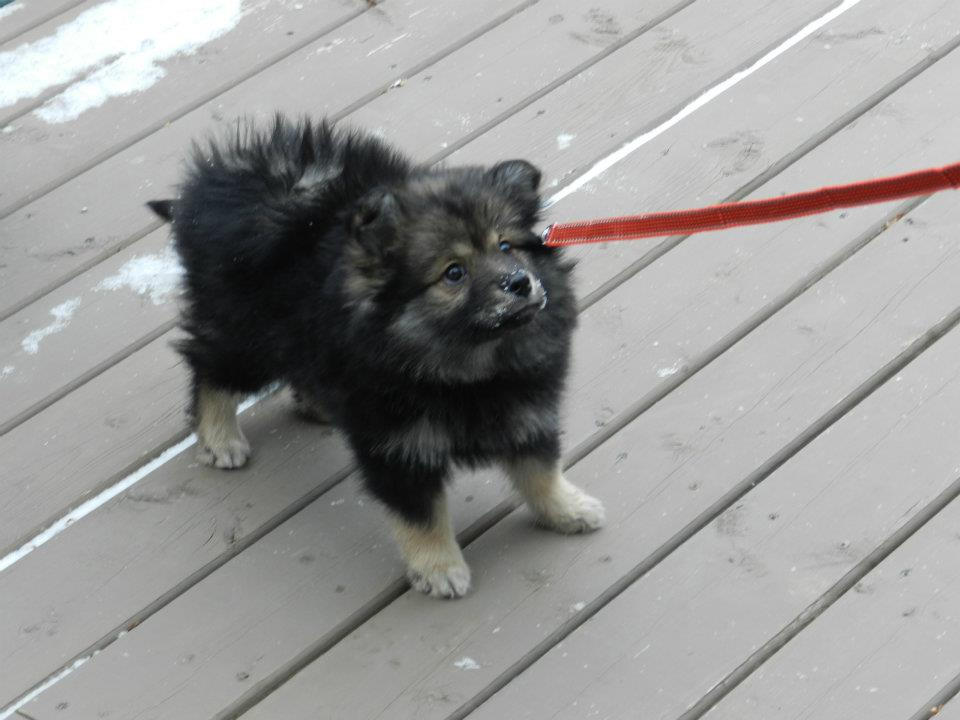
\includegraphics[width=\textwidth]{handout/dog.jpg}
            \caption{My dog}
            \label{fig:my-dog}
        \end{figure}

        Once you've done that. Try adding a 3 high by 3 wide table (including the table headers). Again you can start by typing
        \verb"\begin{table}", then press enter to autocomplete the table template.
        \begin{enumerate}
            \item First just fill out the given 2x2 table and compile it to ensure things are working.
            \item Add the \say{h} as we did for the picture to place the table directly below this list (more or less).
            \item Replace \say{c}s with the letter \say{l} to left-align text
            \item Remove vertical lines by removing the bars \verb"|".
            \item Add one more letter \say{l} to make the table 3 wide
            \item Add \verb"\usepackage{booktabs}" to the preamble.
            \item Use the \verb"\toprule", \verb"\midrule", and \verb"\bottomrule" horizontal lines from the booktabs package to format your table.
            \item Add a caption.
            \item Add a label.
        \end{enumerate}

        % Add table here
        \begin{table}[h]
            \centering
            \begin{tabular}{lll}
            \toprule
                1 & 2 & 3 \\
            \midrule
                4 & 5 & 6 \\
                7 & 8 & 9 \\
            \bottomrule
            \end{tabular}
            \caption{Caption}
            \label{tab:my_label}
        \end{table}

    \lipsum[1]
    
    \section{Referencing}
        Replace the numbers in the list below with references to the appropriate sections, figures, and equations using the \verb"\ref{}" command. You will need to include the \verb"\usepackage[hidelinks]{hyperref}" command in the preamble to make them clickable.


        \begin{itemize}
            \item Section \ref{sec:title} (title).
            \item Figure \ref{fig:my-dog} (dog).
            \item Equation \ref{eq:quadratic} (quadratic).
        \end{itemize}
        

        

        
        
    

\end{document}
